\section{Experimental Results}


\begin{figure*}[!t]
\centering
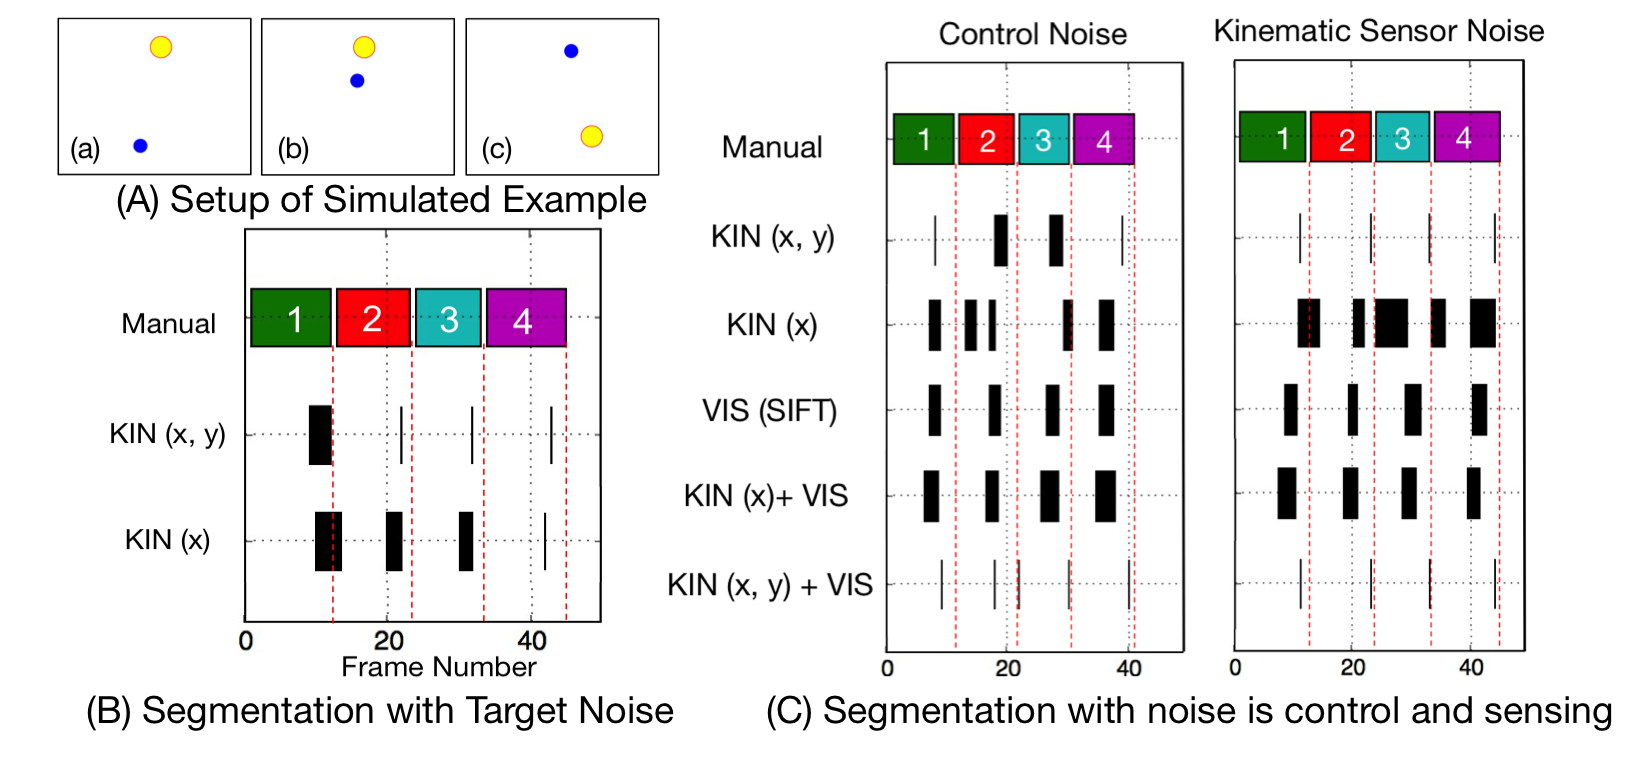
\includegraphics[width=0.8\linewidth]{figures/toyEx}
\caption{The figure shows a simulated example with a robot in blue and target in yellow. The robot moves to the target and a new target appears. In each episode, we have 4 targets in these experiments and each algorithm run uses 5 episodes. The first row shows the manual segmentation -- reaching each target. Subsequent rows illustrate learn segmentation without supervision under various combinations of input data.  
Each row is a sequence of transitions represented by blocks. The width of every block represents the confidence interval conveying the length of transition, with some transitions being sharp while others are longer.\todo{flesh out}}
\label{fig:toyEx}
\vspace{-15pt}
\end{figure*}

\todo{Explain the method, add algorithm block and work through the simulated example}

\subsection{Synthetic Example}
A Synthetic example with a robot in blue and target in yellow is shown in \figref{toyEx}. The robot moves to the target, and a new target appears after that robot has reached the current target. For the example, we have 4 targets. For each demonstration episode, the target $i$ is sampled from  $\sim\,\mathcal{N}(\mu_i, 1)$ where $\mu_i$ is randomly generated in the first episode and maintained constant across subsequent episodes. For these example, we generate 5 episodes of each individual test.

\figref{toyEx} (b) shows the results of unsupervised segmentation into the 4 steps -- each time the robot reaches the target, using only kinematics data ($\binom{x(t)}{y(t)}$). The results for this preliminary example align the transitions with changes in directions robots motions affirming out model for hierarchical clustering. 

We further evaluate the effect of partial observability, by reducing the state dimension to only $(x(t))$. As expected, the our method only has a component of the gradient, and hence the uncertainty on the output transitions increases, albeit around the correct mean. 

Next, we introduce control noise in the system, $x(t+1) = x(t)+u(t)+\nu$, where $\nu\, \sim\, \mathcal{N}(0, d_1)$ where varying $d_1\in[0,1]$. The \figref{toyEx} (c) shows the results for $d_1=0.25$. Similar to the previous experiment we experiment with full kinematics along with partial observability. We find that in case of noise, one dimensional trajectory can have drifts which would erroneously show up as transitions. 
We also evaluate the performance of segmentation using only Visual features, specifically SIFT features. We observe that the segments are correctly identified, however due to the nature of SIFT feautures, transitions have longer time lengths.
Finally, we note that a combination of Kinematics and Visual features allows disambiguation from noise, and hence allows for sharper transition clusters than either of those independently. 

Next, we introduce a kinematic sensor noise in the system $\hat{x}(t)= x(t)+\nu$, where $\nu\, \sim\, \mathcal{N}(0, d_2)$ where varying $d_2\in[0,1]$. The \figref{toyEx} (c) shows the results for $d_2=0.25$. We note that only the kinematics is corrupted with noise, while the vision sees a perfectly straight trajectory. We first segment using full kinematic state. Thereafter we use partially observed state as in the aforementioned case. We observe that in this case, the segmentation performance substantially degrades. Then, we use SIFT visual features as in previous experiment. We find improved transitions based only on videos. We then combine with partially observed state, this results in slight improvement, and combination with full kinematics state with noise yields drastic improvements in segmentaiton performance. 

%===============================================================

\begin{figure*}[ht!]
	\centering
	\begin{subfigure}[t]{3.4in}
	    \centering
        
\includegraphics[width=0.5\linewidth]{figures/insert}
		\caption{The figure illustrates the performance of unsupervised segmentation of the 3 Step Lego Assembly Task performed with tele-operated PR2 with two techniques of manual demonstrations.}
		\figlabel{lego-pr2}
		\vspace{-5pt}
	\end{subfigure}
	 \hspace{0.1in}
	\begin{subfigure}[t]{3.4in}
	    \centering
		
\includegraphics[width=0.5\linewidth]{figures/insert}
		\caption{The figure illustrates the comparison of unsupervised segmentation of the Toy Example performed with tele-operated PR2 with two techniques of manual demonstrations.}
		\figlabel{toyPlane-pr2human}
		\vspace{-5pt}
	\end{subfigure}
	\caption{\todo{fix figure}}
	\figlabel{pr2_expts}
	\vspace{-15pt}
\end{figure*}

\subsection{PR2: Legos and Toy Plane Assembly}
% \begin{figure}[!t]
% \centering
% 
\includegraphics[width=\linewidth]{figures/insert.png}
% \caption{The figure illustrates the performance of unsupervised segmentation of the 3 Step Lego Assembly Task performed with tele-operated PR2 with two techniques of manual demonstrations.}
%  \label{fig:lego-pr2}
% \vspace{-10pt} 
% \end{figure}
\figref{lego-pr2}, \figref{pr2_toyplane}


\subsection{Human Demonstration of Toy Plane Assembly}
% \begin{figure}[!t]
% \centering
% 
\includegraphics[width=\linewidth]{figures/insert.png}
% \caption{The figure illustrates the comparison of unsupervised segmentation of the Toy Example performed with tele-operated PR2 with two techniques of manual demonstrations.}
%  \label{fig:toyPlane-pr2human}
% \vspace{-10pt} 
% \end{figure}
\figref{toyPlane-pr2human}


%===============================================================

\subsection{Surgical Subtask Segmentation}

We apply our method to the JIGSAWS dataset\cite{gao2014jigsaws} consisting of surgical activity for human motion modeling. The dataset was captured using the da Vinci Surgical System from eight surgeons with different levels of skill performing five repetitions each of suturing and needle passing.

\vspace{0.5em}
\noindent\textbf{Suturing: }Next, we explored 39 examples of a 4 throw suturing task (\figref{suturing}). Using the right arm, the first step is to penetrate one of the points on right side. The next step is to force the needle through the phantom to the other side. Using the left arm, the robot pulls the needle out of the phantom, and then hands it off to the right arm for the next point. 


\vspace{0.5em}
\noindent\textbf{Needle Passing: } We applied our framework to 28 demonstrations of the needle passing task.
The robot passes a needle through a loop using its right arm, then its left arm to pull the needle through the loop. Then, the robot hands the needle off from the left arm to the right arm. This is repeated four times as illustrated with a manual segmentation in 
\figref{needlePassing}.

\todo{Table of Results}\\
\todo{Description of metric} from watch n patch paper. Otherwise use Dynamic Time warping to match transitions.


\subsection{Evaluation of Results }

\noindent \textit{Exp1. End-to-end result with some task}

\begin{enumerate}
\item Show that clusters are sensible and align with some intuitive criteria e.g., surgemes
\end{enumerate}

\noindent \textit{Exp2. Does Vision Help}

\begin{enumerate}
\item Remove visual features and show that clusters degrade
\end{enumerate}

\noindent \textit{Exp3. Parameter Search}

\begin{enumerate}
\item Describe our eval procedure and how we arrived at the architecture we did.
\end{enumerate}

\noindent \textit{Robustness}
\begin{enumerate}
\item Add noise or corrupt images and test to see how robust the segmentations we learn are.
\end{enumerate}


\begin{figure*}[!ht]
	\centering
	\begin{subfigure}[t]{3.4in}
	    \centering
        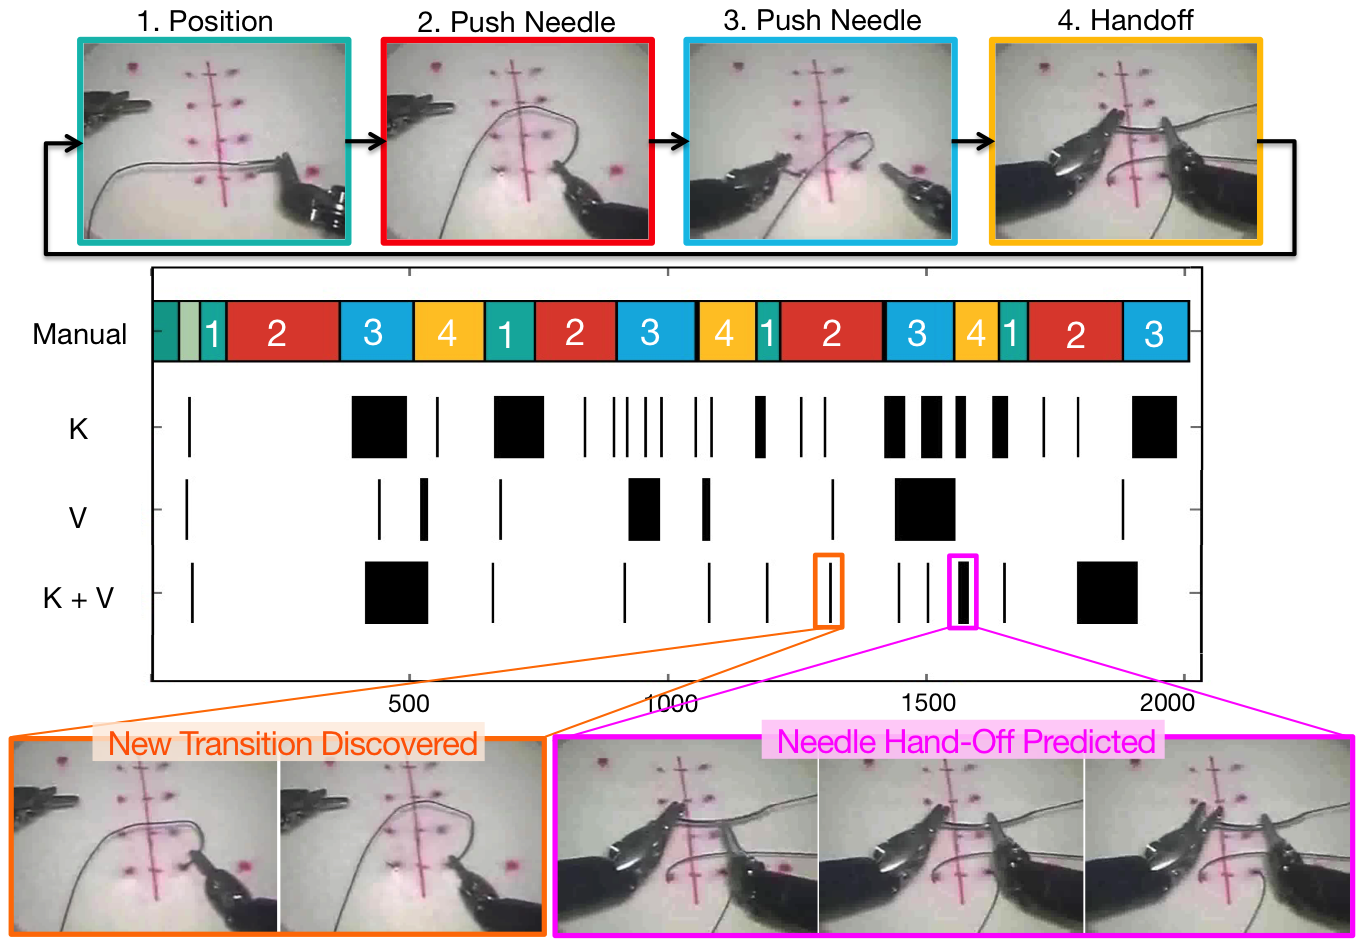
\includegraphics[width=\linewidth]{figures/suturing}
		\caption{Suturing}
		\label{fig:suturing}
		\vspace{-5pt}
	\end{subfigure}
	 \hspace{0.1in}
	\begin{subfigure}[t]{3.4in}
	    \centering
		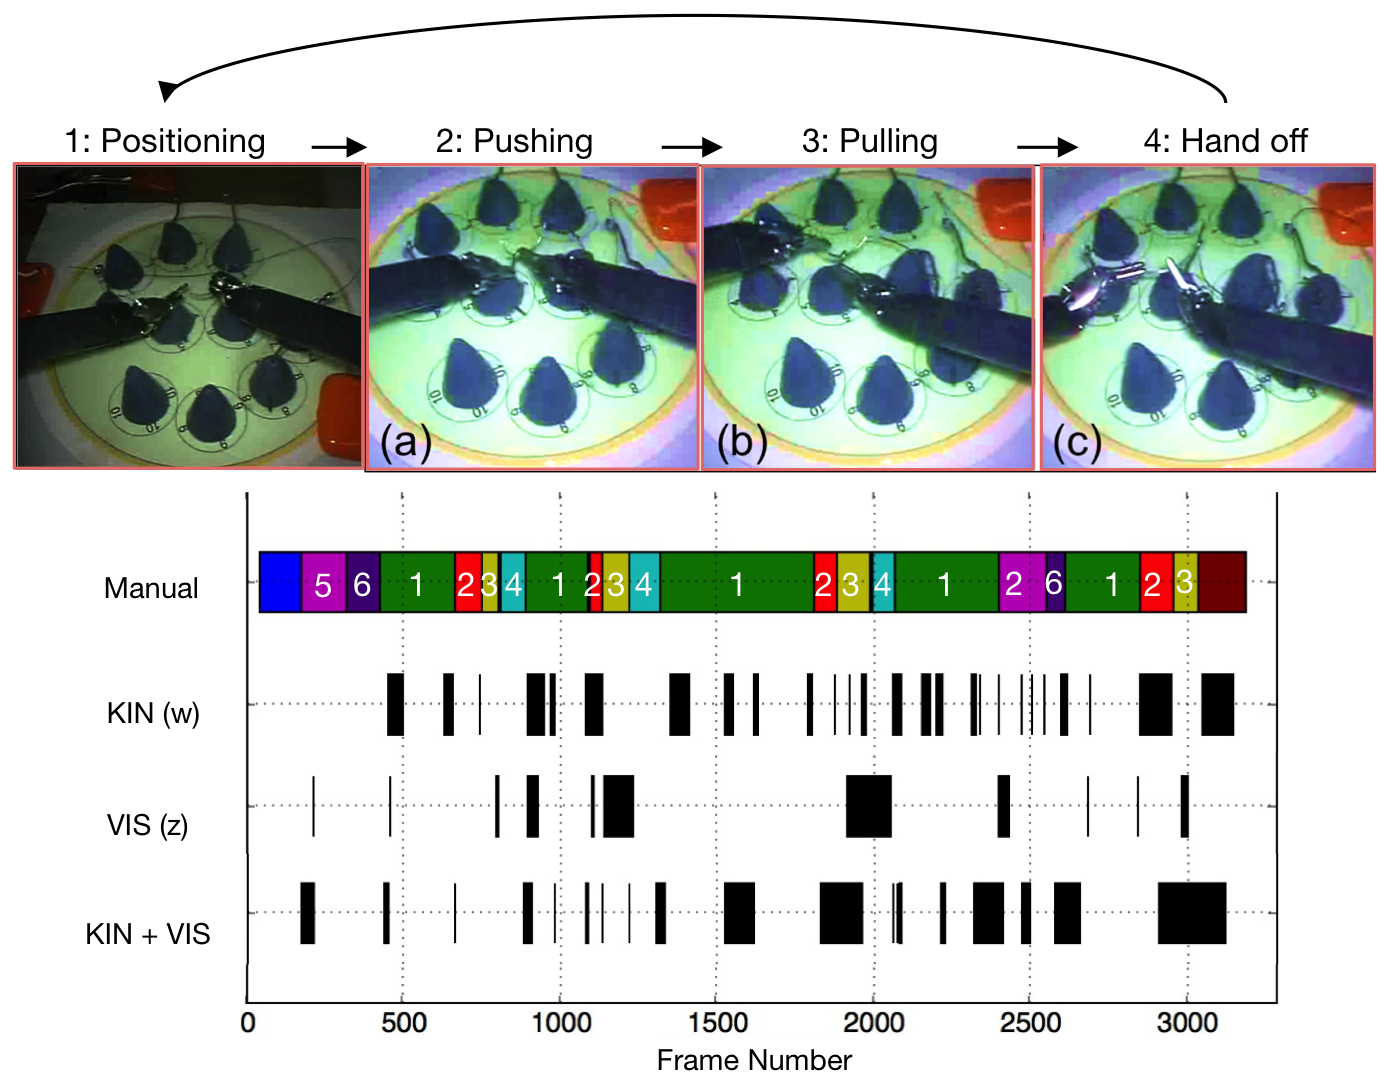
\includegraphics[width=\linewidth]{figures/needle_passing}
		\caption{Needle Passing}
		\label{fig:needlePassing}
		\vspace{-5pt}
	\end{subfigure}
	\caption{\todo{fix figure} The figure shows a sequence of images for the Suturing and Needle Passing tasks in JIGSAWS dataset\cite{gao2014jigsaws}.
The first row shows a manual segmentation of the task in 4 semantic steps: (1) Needle Positioning, (2) Needle Pushing, (3) Pulling Needle, (4) Hand-off.
Both these tasks require 4 repetitions of the full 4 step cycle and run for approx. 100s (frame numbers are at 30 fps). 
We use 5 expert demonstrations in each case, and it is worth noting that there are multiple spurious segments in needle passing task such as (5) Moving to Center with Needle and (6) Re-orienting Needle. We show the sub-task level segmentation results from our completely unsupervised approach with only Kinematics, only visual data and a concatenation of both.}
	\label{fig:sensitivityAnalysis}
	\vspace{-15pt}
\end{figure*}


\subsection{Discussion}
\begin{enumerate}
\item How successful was our unsupervised approach in learning meaningful segmentations
\item RGB videos vs. RGB-D videos
\end{enumerate}

